\cleardoublepage
\chapter{Test classici della Relatività Generale}
\label{cha:testclassici_rg}

\section{I test classici della Relatività Generale}
\label{sec:verififiche-relativita}

Adottando la metrica di Schwarzschild siamo in grado di fare delle previsioni
teoriche riguardo alcuni fenomeni osservabili nel sistema solare. Queste sono
state confermate sperimentalmente e hanno permesso il riconoscimento della
validità della teoria della relatività generale.

\subsection{Precessione del perielio}
\label{sec:precessione-perielio}

\begin{figure}
  \centering
  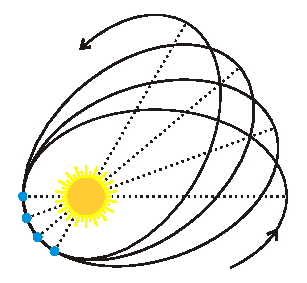
\includegraphics{figure/Perihelion_precession}
  \caption[Precessione del perielio di un pianeta]{Precessione del perielio di
    un pianeta.
    {\footnotesize (Crediti: Mpfiz
      \url{https://commons.wikimedia.org/wiki/File:Perihelion_precession.svg})}}
  \label{fig:precessione-perielio}
\end{figure}

La prima legge di Keplero afferma che l'orbita descritta dai pianeti è
un'ellisse.  Questo risultato è rigorosamente vero nel caso in cui il pianeta
interagisce solo con la stella intorno a cui orbita.  La presenza di altri
eventuali pianeti perturba il sistema facendo in modo che l'orbita non sia
chiusa ma piuttosto una rosetta, si ha quindi una precessione del perielio, come
rappresentato nella figura~\ref{fig:precessione-perielio}.  Per esempio, dalle
osservazioni astronomiche si è scoperto che il perielio di Mercurio si sposta di
circa \ang{;;575} ogni cento anni.  Utilizzando la meccanica newtoniana e
tenendo conto della presenza di tutti i pianeti conosciuti si prevede una
precessione del perielio di Mercurio pari a circa \ang{;;532}.  Per spiegare
questa incongruenza sono state proposte diverse ipotesi, fra cui la presenza di
un corpo perturbante come un nuovo pianeta (Vulcano), più interno di Mercurio, o
un satellite di Mercurio.  Tuttavia questi corpi non sono mai stati trovati e
faremo vedere che la relatività generale è in grado di risolvere questo
problema.

% TODO: capire per bene i passaggi dell'Adler
Per determinare l'orbita di un pianeta abbiamo bisogno di quattro equazioni per
le quattro coordinate spazio-temporali sferiche $t$, $r$, $\theta$ e $\phi$.
Una prima equazione differenziale per la coordinata $r$ si ottiene dividendo
l'intervallo di tempo proprio di Schwarzschild~\eqref{eq:metrica-schwarzschild}
per $\dd\tau^{2}$
\begin{equation}
  \label{eq:mercurio-r}
  \bigg(\toder{\tau}{\tau}\bigg)^{2} = 1 = \bigg(1 -
  \frac{r_{\textup{S}}}{r}\bigg)\dot{t}^{2} - \bigg(1 -
  \frac{r_{\textup{S}}}{r}\bigg)^{-1}\dot{r}^{2} - r^{2}(\dot{\theta}^{2} +
  \sin^{2}\theta \dot{\phi}^{2}).
\end{equation}
Il punto sopra le variabili indica la derivazione rispetto al tempo proprio
$\tau$.  Per determinare le altre equazioni dobbiamo risolvere il problema
variazionale
\begin{equation}
  \delta \int \dd \tau = 0
\end{equation}
in cui $\dd\tau$ è la metrica di Schwarzschild.  Questo problema può essere
risolto più facilmente considerando la seguente formulazione equivalente
\begin{equation}
  \begin{split}
    \delta\int \dd\tau &= \delta \int \bigg(\toder{\tau}{\tau}\bigg)^{2} \dd
    \tau \\
    &= \delta \int \bigg(\bigg(1 - \frac{r_{\textup{S}}}{r}\bigg)\dot{t}^{2} -
    \bigg(1 - \frac{r_{\textup{S}}}{r}\bigg)^{-1}\dot{r}^{2} -
    r^{2}(\dot{\theta}^{2} + \sin^{2}\theta \dot{\phi}^{2}) \bigg) \dd \tau = 0.
  \end{split}
\end{equation}
Da qui, considerando la funzione integranda come una lagrangiana, si ottengono
tre equazioni di Eulero-Lagrange per le coordinate, rispettivamente, $\theta$,
$\phi$ e $t$
\begin{subequations}
  \begin{gather}
    \toder{}{\tau}(r^{2}\dot{\theta}) = r^{2}\sin\theta\cos\theta
    \dot{\phi}^{2}, \label{eq:mercurio-mu} \\
    \toder{}{\tau}(r^{2} \sin^{2}\theta \dot{\phi}) = 0, \label{eq:mercurio-phi}
    \\
    \toder{}{\tau}\bigg(\bigg(1 - \frac{r_{\textup{S}}}{r}\bigg) \dot{t} \bigg)
    = 0. \label{eq:mercurio-t}
  \end{gather}
\end{subequations}
Non abbiamo scritto l'equazione di Eulero-Lagrange per la coordinata $r$ poiché
utilizzeremo la~\eqref{eq:mercurio-r}.

Allo stesso risultato si giunge considerando l'equazione della geodetica
\begin{equation}
\frac{d^2 x^{\mu}}{d\tau^2}+\Gamma^{\mu}_{\nu\rho}\frac{dx^{|nu}}{d\tau}
\frac{d x^{_\rho}}{d \tau} = 0
\end{equation}
in cui gli elementi della connessione affine sono calcolati a partire dalla
metrica di Schwarzshild. In particolare le tre equazioni precedenti sono
ottenute ponendo nella equazione della geodetica $\mu=2$, $\mu=3$ e $\mu=0$,
rispettivamente.

Notiamo che associando all'equazione differenziale~\eqref{eq:mercurio-mu} le
condizioni iniziali $\theta = \pi/2$ e $\dot{\theta} = 0$, la funzione costante
$\theta(\tau) = \pi/2$ costituisce l'unica soluzione di questo problema di
Cauchy.  Ciò significa che con un'opportuna scelta delle coordinate il moto del
pianeta si svolge in un piano, così come succede anche in meccanica classica.
Sostituendo $\theta = \pi/2$ nella~\eqref{eq:mercurio-phi} abbiamo
\begin{equation}
  \label{eq:mercurio-phi2}
  \toder{}{\tau}(r^{2}\dot{\phi}) = 0 \implies r^{2}\dot{\phi} = h =
  \text{costante}
\end{equation}
cioè il pianeta si muove con velocità areolare costante, come nel problema di
Keplero classico.  Invece dalla~\eqref{eq:mercurio-t} otteniamo
\begin{equation}
  \label{eq:mercurio-t2}
  \bigg(1 - \frac{r_{\textup{S}}}{r}\bigg)\dot{t} = l = \text{costante}.
\end{equation}
Sostituendo tutti questi risultati nella~\eqref{eq:mercurio-r} troviamo
\begin{equation}
  \label{eq:mercurio-r2}
  1 = \bigg(1 - \frac{r_{\textup{S}}}{r}\bigg)^{-1}l^{2} - \bigg(1 -
  \frac{r_{\textup{S}}}{r}\bigg)^{-1}\dot{r}^{2} - \frac{h^{2}}{r^{2}}.
\end{equation}

Per determinare l'equazione dell'orbita conviene porre
$r = r(\phi)$, quindi indicando con l'apice la derivazione rispetto a
$\phi$ abbiamo
\begin{equation}
  \dot{r} \equiv  \toder{r}{\tau} = \toder{r}{\phi} \toder{\phi}{\tau} = r'
  \dot{\phi} = r' \frac{h}{r^{2}}
\end{equation}
e ponendo $u = 1/r$, con
\begin{equation}
  \dot{r} \equiv \frac{h}{r^{2}}r' = \frac{h}{r^{2}}\toder{r}{\phi} =
  hu^{2}\toder{}{\phi} \frac{1}{u} = -hu^{2}\frac{u'}{u^{2}} = -hu'.
\end{equation}

Allora la~\eqref{eq:mercurio-r2} diventa
\begin{equation}
  1 - r_{\textup{S}}u = l^{2} - h^{2}u'^{2} - h^{2}u^{2}(1 - r_{\textup{S}}u),
\end{equation}
da cui, riarrangiando,
\begin{equation}
  \label{eq:mercurio-u'}
  u'^{2} = \frac{l^{2} - 1}{h^{2}} + \frac{r_{\textup{S}}}{h^{2}}u - u^{2} +
  r_{\textup{S}}u^{3} \equiv f(u).
\end{equation}
Questa equazione può essere integrata nel seguente modo
\begin{equation}
  \toder{u}{\phi} = \sqrt{f(u)} \implies \dd\phi = f^{-1/2}(u) \dd u \implies
  \phi = \phi_{0} + \int_{u_{0}}^{u} f^{-1/2}(\tilde{u}) \dd \tilde{u}.
\end{equation}

Sebbene questa sia la soluzione esatta, essa non è utile a livello pratico
perché fornisce solo un'espressione implicita di $u$, e quindi $r$, rispetto a
$\phi$.  Nella risoluzione del problema di Keplero classico si giunge
all'equazione di Binet che è un'equazione differenziale del secondo ordine in
$u$.

Allora per ottenere un'equazione differenziale del secondo ordine in $u$ da
confrontare con l'equazione di Binet, conviene derivare rispetto a $\phi$
la~\eqref{eq:mercurio-u'}.  Abbiamo
\begin{equation}
  \label{eq:mercurio1}
  2u'u'' = \frac{r_{\textup{S}}}{h^{2}}u' - 2uu' + 3r_{\textup{S}}u^{2}u'
  \implies u'\bigg(2u'' - \frac{r_{\textup{S}}}{h^{2}} + 2u -
  3r_{\textup{S}}u^{2}\bigg) = 0.
\end{equation}
Una soluzione di questa equazione è $u' = 0$, cioè $u(\phi) = 1/r(\phi) =
\text{costante}$.  Tuttavia questa situazione non ci interessa poiché descrive
un moto circolare, essendo la distanza dal centro del campo costante, quindi non
c'è un perielio e non è possibile osservare la sua precessione.  L'altra
possibile soluzione è
\begin{equation}
  \label{eq:binet-relativ}
  2u'' - \frac{r_{\textup{S}}}{h^{2}} + 2u - 3r_{\textup{S}}u^{2} = 0 \implies
  u'' + u = \frac{r_{\textup{S}}}{2h^{2}} + \frac{3}{2}r_{\textup{S}}u^{2} =
  \frac{GM}{r^{4}(\ltoder{\phi}{\tau})^{2}} + \frac{3}{2}r_{\textup{S}}u^{2},
\end{equation}
in cui $M$ è la massa del corpo che genera il campo gravitazionale.

Nel problema di Keplero classico, l'\index{equazione!di Binet}equazione di Binet
è
\begin{equation}
  \label{eq:binet}
  u'' + u = \frac{GM}{r^{4}(\ltoder{\phi}{t})^{2}}.
\end{equation}

Nella eq. relativistica osserviamo per prima che per piccole velocità
$\ltoder{\phi}{\tau} \approx \ltoder{\phi}{t}$.  Inoltre per i pianeti del
sistema solare risulta
\begin{equation}
  \frac{3r_{\textup{S}}u^{2}/2}{r_{\textup{S}}/(2h^{2})} = 3u^{2}h^{2} \ll 1,
\end{equation}
poiché
\begin{equation}
  3u^{2}h^{2} = \frac{3}{r^{2}}r^{4} \bigg(\toder{\phi}{\tau}\bigg)^{2} = 3r^{2}
  \bigg(\toder{\phi}{\tau}\bigg)^{2} \approx 3 v_{\textup{t}}^{2},
\end{equation}
in cui $v_{\textup{t}} = r\ltoder{\phi}{t}$ è la velocità tangenziale del corpo,
espressa in unità di $c$ poiché abbiamo posto $c = 1$.  Per Mercurio, il pianeta
più interno del sistema solare e quindi con la maggior velocità tangenziale,
$3 v_{\textup{t}}^{2} = \num{7.7e-8}$, quindi possiamo considerare il termine
$3r_{\textup{S}}u^{2}/2$ nella~\eqref{eq:binet-relativ} come una debole
perturbazione.  In dettaglio, vogliamo risolvere l'equazione
\begin{equation}
  u'' + u = A + \frac{\epsilon u^{2}}{A},
\end{equation}
con $A = r_{\textup{S}}/(2h^{2})$ e $\epsilon = 3Ar_{\textup{S}}/2  \ll 1$.
Cerchiamo soluzioni del tipo
\begin{equation}
  u(\phi) = u_{0}(\phi) + \epsilon v(\phi),
\end{equation}
con $u_{0}(\phi)$ soluzione dell'equazione di Binet classica
\begin{equation}
  \label{eq:binet-2}
  u_{0}'' + u_{0} = A
\end{equation}
cioè
\begin{equation}
  u_{0} = A + B\cos(\phi + \phi_{0}),
\end{equation}
con $B$ e $\phi_{0}$ costanti reali di integrazione.  Ruotando opportunamente il
sistema di riferimento si può fare in modo che $\phi_{0} = 0$ cosicché $u_{0}$
diventa
\begin{equation}
  \label{eq:sol-binet}
  u_{0}(\phi) = A + B\cos\phi.
\end{equation}
Dunque l'equazione da risolvere è
\begin{equation}
  (u_{0}'' + \epsilon v'') + (u_{0} + \epsilon v) = A + \epsilon \frac{(u_{0} +
    \epsilon v)^{2}}{A} = A + \epsilon \frac{u_{0}^{2}}{A} +
  \mathcal{O}(\epsilon^{2}).
\end{equation}
Tenendo conto della~\eqref{eq:binet-2} l'equazione per $v(\phi)$ al primo ordine
in $\epsilon$ è
\begin{equation}
  \begin{split}
    v'' + v &= \frac{u_{0}^{2}}{A} = A + 2B\cos\phi +
    \frac{B^{2}}{A}\cos^{2}\phi \\
    &= \bigg(A + \frac{B^{2}}{2A}\bigg) + 2B\cos\phi +
    \frac{B^{2}}{2A}\cos(2\phi),
\end{split}
\end{equation}
in cui abbiamo ricordato l'identità trigonometrica
$\cos^{2}\phi = (1 + \cos(2\phi))/2$.  Dunque questa è l'equazione differenziale
del secondo ordine relativa al termine che perturba l'orbita dei pianeti.
Questa equazione è lineare, quindi la soluzione può essere espressa come somma
delle soluzioni delle tre equazioni seguenti
\begin{subequations}
  \begin{align}
    v_{a}'' + v_{a} &= A + \frac{B^{2}}{2A} \implies v_{a}(\phi) = A +
    \frac{B^{2}}{2A}, \\
    v_{b}'' + v_{b} &= 2B\cos\phi \implies v_{b}(\phi) = B\phi \sin\phi, \\
    v_{c}'' + v_{c} &= \frac{B^{2}}{2A}\cos(2\phi) \implies v_{c}(\phi) =
    -\frac{B^{2}}{6A}\cos(2\phi),
  \end{align}
\end{subequations}
dunque
\begin{equation}
  v(\phi) = v_{a}(\phi) + v_{b}(\phi) + v_{c}(\phi) = A + \frac{B^{2}}{2A} +
  B\phi\sin\phi - \frac{B^{2}}{6A}\cos(2\phi)
\end{equation}
e in questo modo $u(\phi)$ è data da
\begin{equation}
  \begin{split}
    u(\phi) &= u_{0}(\phi) + \epsilon v(\phi) \\
    &= A + B\cos\phi + \epsilon A + \frac{\epsilon B^{2}}{2A} + \epsilon
    B\phi\sin\phi - \frac{\epsilon B^{2}}{6A}\cos(2\phi).
  \end{split}
\end{equation}
Al primo ordine in $\epsilon$ abbiamo
\begin{equation}
  \cos(\phi - \epsilon\phi) = \cos\phi \cos(\epsilon\phi) + \sin\phi
  \sin(\epsilon\phi) \approx \cos\phi + \epsilon\phi\sin\phi,
\end{equation}
allora
\begin{equation}
  \frac{1}{r(\phi)} = u(\phi) \approx A + B\cos(\phi - \epsilon\phi) +
  \epsilon\bigg(A + \frac{B^{2}}{2A} - \frac{B^{2}}{6A}\cos(2\phi)\bigg).
\end{equation}
L'ultimo termine, fra parentesi, induce una piccola variazione nella distanza
radiale del pianeta, ma non può essere responsabile della precessione del
perielio poiché il termine $\cos(2\phi)$ ha periodo sottomultiplo intero di
$2\pi$ (quindi dopo un'intera rivoluzione di $\var \phi = 2\pi$ assume di nuovo
lo stesso valore).  Il resto della funzione $u(\phi)$ si differenzia dalla
soluzione~\eqref{eq:sol-binet} dell'equazione di Binet per la presenza di
$-\epsilon\phi$ nell'argomento del coseno.

 Il perielio si ha quando $r(\phi)$ è
minimo, vale a dire quando $u(\phi)$ è massimo e ciò si verifica quando il
coseno del secondo termine vale $1$, cioè quando
\begin{equation}
  \phi_{n}(1 - \epsilon) = 2\pi n \implies \phi_{n} = \frac{2\pi n}{1 -
    \epsilon} \approx 2\pi n(1 + \epsilon)
\end{equation}
con $n$ numero di rivoluzioni compiute dal pianeta intorno al Sole a partire da
un istante iniziale fissato.  Il perielio successivo si ha dopo una variazione
della coordinata $\phi$ di
\begin{equation}
  \var\phi = \phi_{n+1} - \phi_{n} = 2\pi(1 + \epsilon)
\end{equation}
invece di $2\pi$ come succede per un'orbita chiusa.

La relatività generale prevede allora una precessione del perielio dei pianeti
nel loro moto intorno al Sole, indipendentemente dalla presenza perturbatrice di
altri corpi.  Stimiamo il valore $\delta\phi$ di questa precessione per
verificare se è in accordo con i dati sperimentali.  Per i pianeti del sistema
solare $r_{\textup{S}} = 2GM_{\odot}$ è il raggio di Schwarzschild del Sole,
allora
\begin{equation}
  \delta\phi = 2\pi\epsilon = 2\pi \frac{3}{4}\frac{r_{\textup{S}}^{2}}{h^{2}} =
  6\pi \frac{G^{2}M_{\odot}^{2}}{h^{2}}.
\end{equation}
In particolare per il pianeta Mercurio si ha
\begin{equation}
  \delta\phi = \ang{;;0.1036}
\end{equation}
e la precessione dopo cento anni, ricordando che il suo periodo orbitale è di
$87.8$ giorni, è data da
\begin{equation}
  \delta_{100}\phi = \frac{\delta\phi \cdot 100 \cdot 365.25}{87.8} =
  \ang{;;43}.
\end{equation}
All'inizio della sezione abbiamo ricordato che la precessione secolare di
Mercurio è di circa \ang{;;575}, possiamo ora concludere che di questi, circa
\ang{;;43} sono dovuti a effetti di relatività generale e circa \ang{;;532} alla
perturbazione indotta dalla presenza degli altri pianeti.  Mercurio è il pianeta
del sistema solare per il quale la precessione relativistica del perielio è più
evidente in quanto è il più interno e quindi il più influenzato dal campo
gravitazionale del Sole.

\subsection{Deflessione della luce}
\label{sec:deflessione-luce}

Secondo la teoria newtoniana, solo i corpi dotati di massa sono soggetti
all'attrazione gravitazionale.  In questo paragrafo vedremo che un fotone (così
come qualsiasi corpo privo di massa a riposo ma dotato di energia) risente della
presenza di un campo gravitazionale, come quello generato dal Sole, deviando la
propria traiettoria.  Questo fenomeno è comprensibile ricordando che tutti i
corpi si muovono lungo geodetiche in uno spazio-tempo curvo.

In relatività speciale, per due eventi separati da un intervallo di tipo luce la
distanza vale $\dd\tau^{2} = 0$ e assumiamo che lo stesso valga anche in
relatività generale.  Assumiamo inoltre che l'equazione della
geodetica~\eqref{eq:geodetica} sia valida anche per le particelle prive di massa
a riposo ma dotate di energia, come i fotoni.  Tuttavia dobbiamo fare attenzione
al fatto che, proprio in virtù del fatto che $\dd\tau^{2} = 0$, non possiamo
parametrizzare la linea d'universo di un fotone, o di una qualsiasi particella
con massa nulla, usando il tempo proprio $\tau$.  Piuttosto dobbiamo utilizzare
un differente parametro $q$ tale che l'equazione della geodetica
\begin{equation}
  \toder[2]{x^{\mu}}{q} + \tensor{\Gamma}{^{\mu}_{\lambda\nu}}
  \toder{x^{\lambda}}{q} \toder{x^{\nu}}{q} = 0
\end{equation}
abbia senso.  A partire da questa equazione si possono ricavare nuovamente,
sempre con l'assunzione $\theta = \pi/2$, le relazioni~\eqref{eq:mercurio-phi2}
e \eqref{eq:mercurio-t2}.  La~\eqref{eq:mercurio-r2} va modificata in questo
modo tenendo conto del fatto che $\dd\tau^{2} = 0$
\begin{equation}
  0 = \bigg(1 - \frac{r_{\textup{S}}}{r}\bigg)^{-1}l^{2} - \bigg(1 -
  \frac{r_{\textup{S}}}{r}\bigg)^{-1}\dot{r}^{2} - \frac{h^{2}}{r^{2}}.
\end{equation}
Svolgendo i calcoli in maniera analoga a quanto visto nel paragrafo precedente e
ponendo sempre $u = 1/r$ si arriva all'equazione
\begin{equation}
  u'\bigg(u'' + u - \frac{3}{2}r_{\textup{S}}u^{2}\bigg) = 0.
\end{equation}
Si possono avere due situazioni:
\begin{equation}
  \label{eq:deflessione1}
  u'' + u - \frac{3}{2}r_{\textup{S}}u^{2} = 0,
\end{equation}
oppure
\begin{equation}
  u' = 0 \implies u(\phi) = u_{0} = \text{costante},
\end{equation}
ma quest'ultima soluzione deve essere scartata per ragioni di stabilità.
Osserviamo che si poteva giungere direttamente alla~\eqref{eq:deflessione1}
partendo dalla~\eqref{eq:mercurio1} e ponendo
$\dd\tau^{2} = 0 \implies 1/h^{2} = (\ltoder{\tau}{\phi})^{2}/r^{4} = 0$.  Il
termine $3r_{\textup{S}}u^{2}/2$ è una piccola perturbazione rispetto a $u$,
infatti
\begin{equation}
  \frac{3r_{\textup{S}}u^{2}/2}{u} = \frac{3r_{\textup{S}}u}{2} =
  \frac{3r_{\textup{S}}}{2r}.
\end{equation}
Considerando il caso del Sole, $r_{\textup{S}} = \SI{3}{\kilo\metre}$ e la
distanza $r$ rispetto alla sua origine a cui un fotone può passare è maggiore o
uguale al raggio $R_{\odot} = \SI{7e5}{\kilo\metre}$, quindi
$3r_{\textup{S}}u^{2}/(2u) \ll 1$.  Allora cerchiamo una soluzione dell'equazione
\begin{equation}
  u'' + u = \epsilon u^{2},
\end{equation}
con $\epsilon = 3r_{\textup{S}}/2$, del tipo
\begin{equation}
  u(\phi) = u_{0}(\phi) + \epsilon v(\phi).
\end{equation}
Sostituendo nell'equazione da risolvere abbiamo
\begin{equation}
  \label{eq:deflessione2}
  u_{0}'' + u_{0} + \epsilon v'' + \epsilon v = \epsilon u_{0}^{2} +
  \mathcal{O}(\epsilon^{2}).
\end{equation}
I termini di ordine zero in $\epsilon$ danno
\begin{equation}
  u_{0}'' + u_{0} = 0,
\end{equation}
la cui soluzione generale è
\begin{equation}
  u_{0}(\phi) = A\cos(\phi + \phi_{0}),
\end{equation}
con $A$ e $\phi_{0}$ costanti di integrazione.  Ruotando il sistema di
coordinate è possibile annullare $\phi_{0}$ cosicché il valore approssimato
$r = 1/u_{0}$ della coordinata radiale soddisfi la relazione
\begin{equation}
  r \cos\phi = \frac{1}{A} = \text{costante}.
\end{equation}
Il prodotto $r\cos\phi$ è la coordinata cartesiana $x$ (vedi
figura~\ref{fig:deflessione-fotone}), quindi questa è l'equazione di una retta
parallela all'asse $y$.  Potevamo attenderci questo risultato: in prima
approssimazione il raggio di luce non viene deviato dal campo gravitazionale del
Sole.  Inoltre la distanza $r_{0}$ di minimo avvicinamento al corpo si ha per
$\cos\phi = 1$, cioè $r_{0} = 1/A \implies u_{0} = (\cos\phi)/r_{0}$.
Uguagliando i termini di ordine uno in $\epsilon$ troviamo
\begin{equation}
  \label{eq:deflessione3}
  v'' + v = u_{0}^{2} = \frac{\cos^{2}\phi}{r_{0}^{2}} = \frac{1 +
    \cos(2\phi)}{2r_{0}^{2}}.
\end{equation}
Cerchiamo soluzioni del tipo
\begin{equation}
  v(\phi) = \alpha + \beta\cos(2\phi)
\end{equation}
con $\alpha$ e $\beta$ costanti di integrazione da determinare.  Sostituendo
nella~\eqref{eq:deflessione3} otteniamo
\begin{equation}
  v'' + v = \alpha - 3\beta\cos(2\phi).
\end{equation}
Confrontando con la~\eqref{eq:deflessione3} abbiamo
\begin{subequations}
  \begin{align}
    \alpha &= \frac{1}{2r_{0}^{2}}, \\
    \beta &= - \frac{1}{6r_{0}^{2}},
  \end{align}
\end{subequations}
quindi
\begin{equation}
  v(\phi) = \frac{1}{2r_{0}^{2}} - \frac{\cos(2\phi)}{6r_{0}^{2}} =
  \frac{2}{3r_{0}^{2}} - \frac{\cos^{2}\phi}{3r_{0}^{2}}.
\end{equation}
In definitiva
\begin{equation}
  \label{eq:deflessione4}
  u(\phi) = u_{0}(\phi) + \epsilon v(\phi) = \frac{\cos\phi}{r_{0}} +
  \frac{2\epsilon}{3r_{0}^{2}} - \frac{\epsilon\cos^{2}\phi}{3r_{0}^{2}}.
\end{equation}

\begin{SCfigure}[1.3]
  \centering
  \begin{tikzpicture}[scale=0.9]
    \draw[fill=white!95!black] (0,0) circle (0.5); % corpo sferico
    \node at (-0.6,0.6) {$M$};
    \draw[-latex,thin] (0,-5) -- (0,5) node[left] {$y$}; % asse y
    \draw[-latex,thin] (0,0) -- (5,0) node[below] {$x$}; % asse x
    % asintoti
    \draw[dashed] (3,-5) node[below] {$O$} node[shape=coordinate] (a) {} --
      (4,0) -- (3,5) node (b) {} node[above] {$S$}
      node[shape=coordinate,pos=0.75] (c) {};
    % traiettoria "vera"
    \draw[bend right=10,thick] ($(a) - (0.1,0)$) to
      node[shape=coordinate,pos=0.65] (e) {} ($(b) - (0.1,0)$);
    % raggio vettore
    \draw[dotted] (0,0) -- node[above] {$r$} (e) node[shape=coordinate,pos=0.4]
      (f) {};
    \path let \p1 = (f) in node[shape=coordinate] (g) at ($(\x1,0)+(0.2,0)$) {};
    \draw[bend right] (g) to node[right] {$\phi$} (f);
    % direzione dell'immagine vista dall'osservatore
    \draw[dotted] (4,0) -- (5,5) node[above] {$S'$}
      node[shape=coordinate,pos=0.75] (d) {};
    \draw[loosely dotted,thin] (4,-5) -- (4,5); % parametro di impatto
    % angolo di deflessione
    \draw[bend left] (c) to node[fill=white,above] {$\Delta = 2\delta$} (d);
    \draw[latex-latex] (0,-4) -- node[fill=white] {$r_{0}$}(4,-4);
  \end{tikzpicture}
  \caption[Deflessione di un fotone nel campo gravitazionale di un corpo
  sferico]{Deflessione di un fotone nel campo gravitazionale di un corpo
    sferico.  La linea continua spessa indica la traiettoria del fotone:
    proviene dalla sorgente $S$ e giunge all'osservatore $O$ dopo essere stato
    deviato dal corpo sferico di massa $M$.  All'osservatore sembrerà che il
    fotone proviene dalla posizione $S'$.  L'angolo $\Delta$ rappresenta la
    deviazione angolare del fotone fra la direzione originaria $S$ e quella
    apparente $S'$.  $r$ è, istante per istante, la distanza fra la posizione
    del fotone e il centro della sorgente del campo gravitazionale, $\phi_{0}$ è
    l'angolo che $r$ forma con l'asse $x$.  $r_{0}$ è la distanza di minimo
    avvicinamento rispetto al corpo sferico, alla quale avviene la deflessione
    del fotone.  Le linee tratteggiate rappresentano gli asintoti della
    traiettoria}
  \label{fig:deflessione-fotone}
\end{SCfigure}
La traiettoria del fotone è, dunque, una retta (data dal termine
$(\cos\phi)/r_{0}$) disturbata da una piccola perturbazione dell'ordine di
$\epsilon$.  Con riferimento alla figura~\ref{fig:deflessione-fotone}, l'effetto
di questa perturbazione è il seguente: il fotone si avvicina al Sole in linea
retta proveniente dalla sorgente $S$, quando l'influenza del campo
gravitazionale della stella non è più trascurabile il fotone viene leggermente
deflesso, quindi si allontana nuovamente in linea retta e giunge all'osservatore
$O$.  Calcoliamo la deflessione del fotone.  Le direzioni asintotiche seguite
dal fotone (linee tratteggiate nella figura~\ref{fig:deflessione-fotone})
corrispondono ai valori di $\phi$ che rendono $r$ infinito, quindi si possono
ottenere calcolando il limite $u \to 0$ nella~\eqref{eq:deflessione4}
\begin{equation}
  0 = \frac{\cos\phi}{r_{0}} + \frac{2\epsilon}{3r_{0}^{2}} -
  \frac{\epsilon\cos^{2}\phi}{3r_{0}^{2}} \implies \cos^{2}\phi -
  \frac{3r_{0}}{\epsilon}\cos\phi - 2 = 0.
\end{equation}
Le soluzioni sono
\begin{equation}
  \cos\phi = \frac{3r_{0}}{2\epsilon}\bigg(1 \pm \sqrt{1 +
    \frac{8\epsilon^{2}}{9r_{0}^{2}}}\bigg),
\end{equation}
ma l'unica accettabile è quella con il segno $-$, poiché quella con il segno $+$
rende il coseno maggiore di $1$.  Sviluppando la soluzione accettabile al primo
ordine in $\epsilon$ abbiamo
\begin{equation}
  \cos\phi = \frac{3r_{0}}{2\epsilon}\bigg(1 - \sqrt{1 +
    \frac{8\epsilon^{2}}{9r_{0}^{2}}}\bigg) \approx
  \frac{3r_{0}}{2\epsilon}\bigg(1 - 1 - \frac{4\epsilon^{2}}{9r_{0}^{2}}\bigg) =
  -\frac{2\epsilon}{3r_{0}} = -\frac{r_{\textup{S}}}{r_{0}}.
\end{equation}
Abbiamo già osservato che per i fotoni che passano nelle vicinanze del Sole
risulta $r_{\textup{S}}/r \ll 1$, quindi $\phi \approx \pm \pi/2$, allora
possiamo porre $\phi = \pi/2 + \delta$, con $\delta \ll 1$, da cui
\begin{equation}
  -\frac{r_{\textup{S}}}{r_{0}} = \cos\phi = \cos(\pi/2 + \delta) = -\sin\delta.
\end{equation}
Dal momento che $\delta$ è molto piccolo possiamo approssimare il seno
dell'angolo con l'angolo stesso e quindi
\begin{equation}
  \delta = \frac{r_{\textup{S}}}{r_{0}}.
\end{equation}
Abbiamo trovato che gli asintoti della traiettoria del fotone formano un angolo
$\delta$ rispetto alla retta di equazione $x = r_{0}$.  La deflessione totale
$\Delta$ è il doppio di questo angolo, dunque, ripristinando il valore della
velocità della luce,
\begin{equation}
  \Delta = 2\delta = \frac{2r_{\textup{S}}}{r_{0}} = \frac{4GM}{c^{2}r_{0}}.
\end{equation}

Per quanto riguarda la deviazione dei raggi di luce da parte del campo
gravitazionale del Sole, supponendo che la distanza di minimo avvicinamento sia
proprio pari al raggio solare $R_{\odot}$, l'angolo di deflessione vale
\begin{equation}
  \Delta_{\odot} = \frac{4GM_{\odot}}{c^{2}R_{\odot}} = \ang{;;1.75}.
\end{equation}
Questa previsione teorica è stata confermata in numerosi esperimenti via via più
accurati, il primo dei quali fu realizzato da Eddington durante l'eclissi totale
di Sole del 1919.

\subsection{Ritardo dei segnali radar}
\label{sec:ritardo-radar}

L'ultimo fenomeno di cui ci interessiamo è il ritardo nel tempo di volo dei
segnali radar rispetto a quanto previsto dalla relatività speciale in uno
spazio-tempo piatto.  Ciò è dovuto al fatto che i fotoni non si muovono lungo
linee rette ma lungo le geodetiche, che hanno lunghezza maggiore rispetto alle
linee rette in uno spazio-tempo piatto.  Questo fenomeno può essere osservato
inviando un segnale radar a un pianeta in congiunzione superiore e misurando il
tempo necessario affinché il segnale vada verso il pianeta e torni sulla Terra.
Tuttavia l'esecuzione di esperimenti su questo fenomeno presentano delle
difficoltà di tipo pratico, delle quali non ci occuperemo.

\begin{figure}
  \centering
  \begin{tikzpicture}
    % Sole.  Il raggio è stato calcolato per tentativi in maniera tale che si
    % intersecasse con la congiungente Terra - Mercurio
    \draw[fill=white!95!black,name path=S] (0,0) circle (1.784) node[above
      left=35] {Sole};
    % Mercurio
    \draw[fill=white!70!black] (1,3) circle (0.5) node[above right=10]
      {Mercurio} node[shape=coordinate] (merc) {};
    % Terra
    \draw[fill=white!70!black] (3,-4) circle (0.5) node[below right=10] {Terra}
      node[shape=coordinate] (terra) {};
    % congiungente Terra - Mercurio
    \draw[dashed,name path=MT] (merc) -- (terra);
    % determino il punto di intersezione fra il Sole e la congiungente Terra -
    % Mercurio
    \path[name intersections={of=S and MT,by={A}}];
    \draw[dashed] (0,0) -- (A);
    \draw[dashed] (merc) -- (0,0) -- (terra);
    \draw[decoration=brace,decorate] (merc) -- node[above, sloped]
      {$\sqrt{r_{2}^{2} - R_{\odot}^{2}}$} (A);
    \draw[decoration=brace,decorate] (A) -- node[above, sloped]
      {$\sqrt{r_{1}^{2} - R_{\odot}^{2}}$} (terra);
    \draw[decoration=brace,decorate] (0,0) -- node[above,sloped] {$r_{2}$}
      (merc);
    \draw[decoration={brace,mirror},decorate] (0,0) -- node[below,sloped]
      {$r_{1}$}  (terra);
    \draw[decoration=brace,decorate] (0,0) -- node[above,sloped] {$R_{\odot}$}
      (A);
  \end{tikzpicture}
  \caption[Schema di un esperimento per la misurazione del ritardo dei segnali
  radar]{Schema di un esperimento per la misurazione del ritardo dei segnali
    radar.  Terra e Mercurio sono in congiunzione superiore.  Le distanze
    riportate sono quelle che si avrebbero se lo spazio-tempo fosse piatto}
  \label{fig:ritardo-radar}
\end{figure}
Senza entrare nei dettagli dei conti forniamo i risultati delle previsioni
teoriche della relatività
generale.\footnote{Questo problema è trattato da
  \textcite[1103-1109]{misner:gravitation};
  \textcite[201-207]{weinberg:gravitation}.}

In un spazio-tempo piatto, il tempo $\tau(r,R_{\odot})$ necessario per un fotone
per giungere tangente sulla superficie del Sole da un punto a distanza $r$ dal
centro della stella è dato semplicemente dal rapporto fra la distanza euclidea
fra questi due punti (vedi figura~\ref{fig:ritardo-radar}) e la velocità dei
fotoni nel vuoto
\begin{equation}
  \tau(r, R_{\odot}) = \frac{\sqrt{r^{2} - R_{\odot}^{2}}}{c}.
\end{equation}
La correzione relativistica per $\tau(r, R_{\odot})$, che tiene conto della
curvatura dello spazio tempo prodotta dal campo gravitazionale del Sole, è
\begin{equation}
  \begin{split}
    t(r,R_{\odot}) &\approx \tau(r,R_{\odot}) + \var t(r,R_{\odot}) \\
    &= \frac{\sqrt{r^{2} - R_{\odot}^{2}}}{c} + \frac{2GM_{\odot}}{c^{3}} \ln
    \frac{r + \sqrt{r^{2} - R_{\odot}^{2}}}{R_{\odot}} +
    \frac{GM_{\odot}}{c^{3}} \sqrt{\frac{r - R_{\odot}}{r + R_{\odot}}}.
  \end{split}
\end{equation}
Il tempo $t_{\textup{tot}}$ totale di volo del fotone per andare dalla Terra, a
distanza $r_{1}$ dal Sole, a un pianeta a distanza $r_{2}$ in congiunzione
superiore è
\begin{equation}
  \begin{split}
    t_{\textup{tot}} &= 2(t(r_{1},R_{\odot}) + t(r_{2},R_{\odot})) \\
    &= 2(\tau(r_{1},R_{\odot}) + \var t(r_{1},R_{\odot}) +
    \tau(r_{2},R_{\odot}) + \var t(r_{2},R_{\odot})).
  \end{split}
\end{equation}
Considerando il sistema Terra-Mercurio, il ritardo
$\var t = 2(\var t(r_{1},R_{\odot}) + \var t(r_{2},R_{\odot}))$ rispetto alla
previsione $2(\tau(r_{1},R_{\odot}) + \tau(r_{2},R_{\odot}))$ in uno
spazio-tempo piatto vale \SI{240}{\micro\second}
(corrispondente ad una distanza di \SI{72}{\kilo\metre})
su un tempo di volo totale $t_{\textup{tot}}$ di
\SI{20}{\minute}.

%%% Local Variables:
%%% mode: latex
%%% TeX-master: "../gravitazione"
%%% fill-column: 80
%%% End:
